\chapter{数据集的构建和预处理}

上一章节提到了验证工具的检测能力需要大量的测试用例,由于合适开源用例的稀缺,合理利用现有无缺陷代码来生成空指针引用缺陷是一种可行的方法。但是,为了方便后续的处理工作,测试用例的选择应该从多维度慎重考虑。然后,为了模型训练的顺利进行,还需要对这些数据进行预处理,构建出正确的控制流图,提取出合适的代码特征。这些工作都是神经网络模型训练所依赖的重要基础。

\section{数据集构建}
\subsection{数据来源}
如果采用从正常代码中构建空指针引用缺陷的方式,首先面对的问题就是选择构建用例的合适的原材料。为了便于后期处理,用例应该包含程序入口,具备语义完整,结构多样化,代码规范简洁等特点,只要程序包含常见的语法结构和调用关系,程序规模不应过大,恰好包含空指针引用陷产生的上下文最佳。依据这些条件,本文选择了部分开源代码数据集作为构建空指针引用缺陷的原始资料,如图\ref{fig:figure4-1}所示。

\begin{figure}
	\centering
	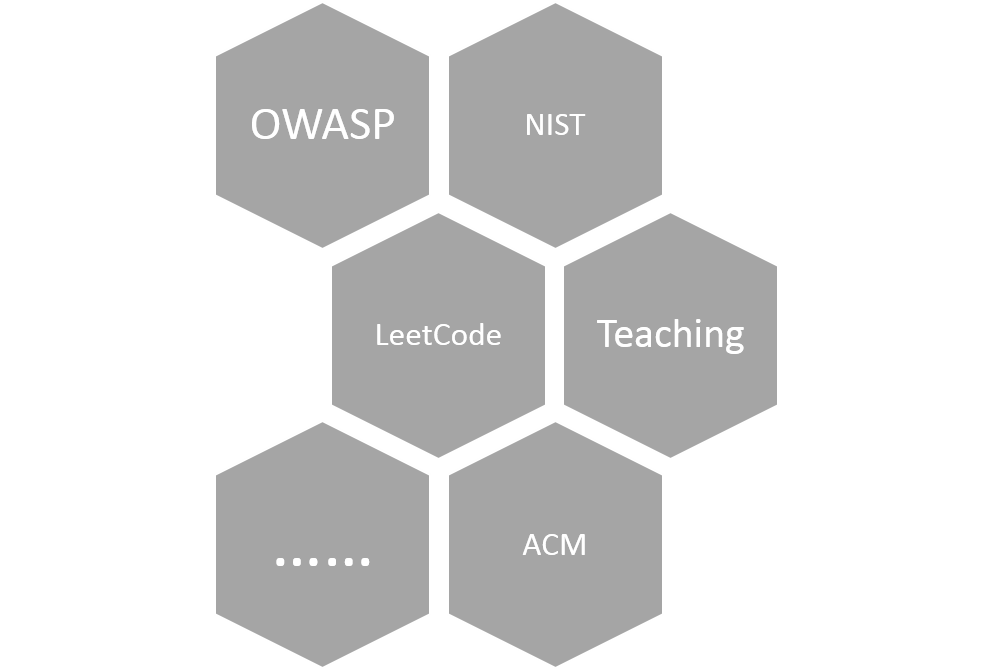
\includegraphics[width=0.70\textwidth]{figures/resource4-1}
	\caption{测试用例来源}\label{fig:figure4-1}
\end{figure}

其中,OWASP[+]和ONIST[+]分别为代码缺陷检测相关领域的项目,从这些项目下可以获得部分标准的空指针引用缺陷用例,同时也可以得到很多具备其他缺陷的测试用例,由于这些用例的代码编写较为规范,并且经过了合理分类,还往往包含说明文档等辅助理解代码的信息,大多都可以用来生成空指针引用缺陷。除此之外,LeetCode和ACM作为编程竞赛性质的项目下也包含大量可以利用的代码,这些代码根据题目的难易级别具备着不同的复杂程度,包含了多样的代码结构,同时,代码的规模往往不大,是作为测试用例生成的良好材料。另外,一些供教学使用的代码也是十分合适的空指针缺陷构造来源,作为补充,本文还添加了部分人工编写的测试用例。

\subsection{测试用例生成}
在取得构造测试用例的原始代码后,需要对这些代码进行检查,确保代码有正确的程序入口,并且可以正确执行。对于OWASP和ONIST项目下的代码,很多用例缺乏Main方法的入口,这会导致后续控制流图提取的困难,这时需要在源代码层级加入合适main方法,调用合适的方法驱动程序的执行。此外,对于ACM和LeetCode项目下的代码资源,虽然所有用例都包含正确的程序入口,但是往往需要合适的输入数据程序才能正确执行。获得这些用例的输入数据并不困难,只需要按照相应题目下的输入输出样子给予输入数据即可驱动程序执行,这些数据的获取可以通过爬虫程序取得,输入数据则可以通过重定向程序的输入流来完成。

空指针引用缺陷的产生必然需要一个产生Null值的缺陷源,在程序的某个位置,变量被赋值为Null随后沿着控制流图向前传播,在遇到解引用时便会触发空指针引用异常。这个变量便是缺陷源,只要在程序中的合适位置构造缺陷源,则有一定的可能会在程序的下文中触发空指针引用缺陷。当用例的可用性得到确认后,需要对用例程序进行语法分析,寻找合适的空指针产生点并构造缺陷源。

对Java文件进行语法分析可以使用Eclipse JDT下的AST来完成,该工具可以在Eclipse环境下获得,利用它能够对Java文件进行解析,生成相应的抽象语法树,并且能够任意修改Java代码的结构和内容。在AST中,Java代码的每一个语法结构都有对应的AST结点表示,这些结点具有完整的层次结构,可以表示整个程序对象到具体方法的某个具体变量。如图\ref{fig:figure4-2}所示,一个for循环的代码片段按照Eclipse AST的标准解析出抽象语法树,表\ref{tab:table4-1}表示部分结点在AST树中对应的名称。

\begin{figure}
	\centering
	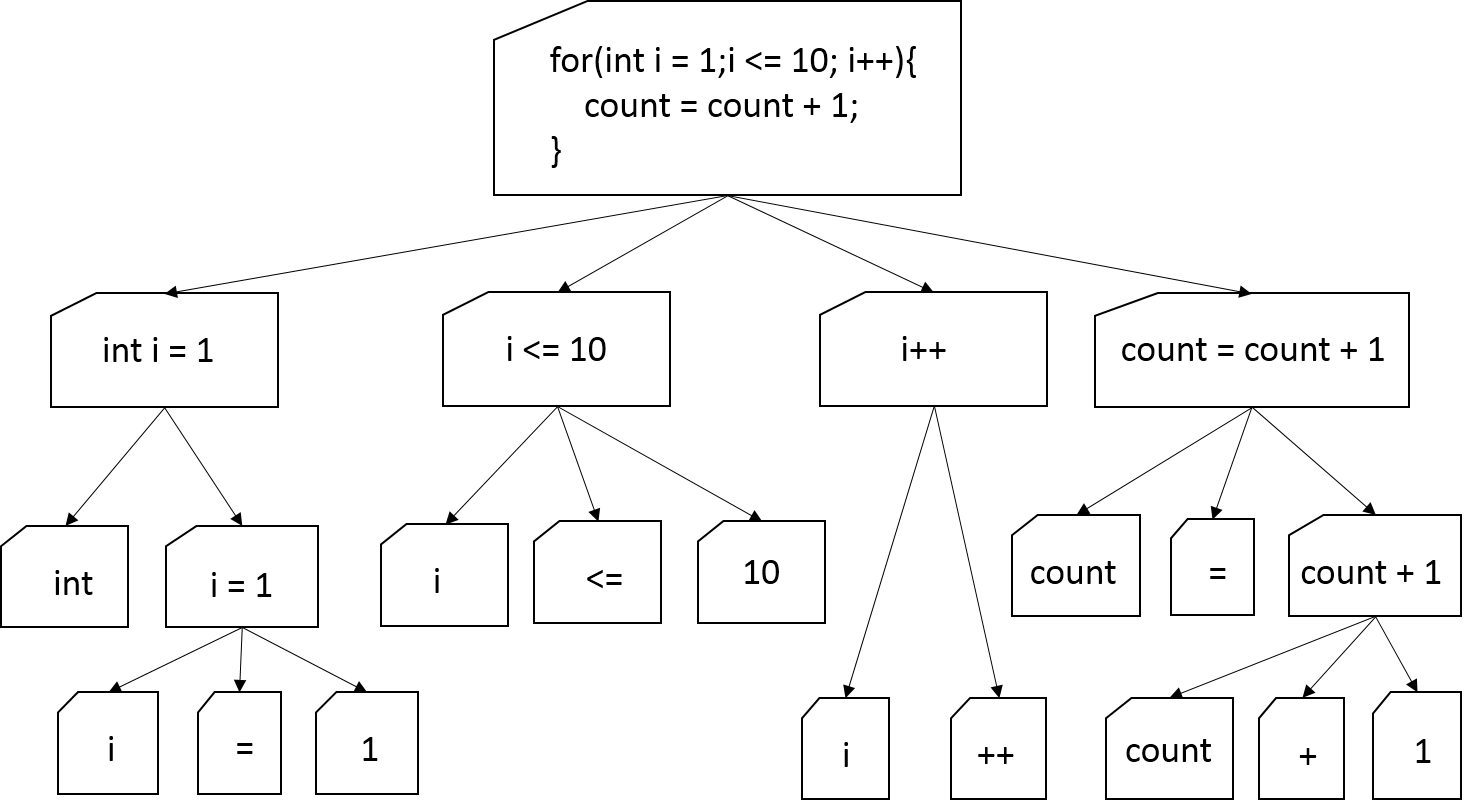
\includegraphics[width=0.70\textwidth]{figures/ast4-2}
	\caption{抽象语法树示例}\label{fig:figure4-2}
\end{figure}

\begin{table}
	\centering
	\caption{AST中的结点信息} \label{tab:table4-1}
	\begin{tabular*}{0.9\textwidth}{@{\extracolsep{\fill}}ccc}
		\toprule
		子节点	&子节点名	&依附于父结点的角色 \\
		\midrule
		int i = 1	&VariableDeclarationExpression	&INITIALIZERS \\
		i <= 10	&InfixExpression	&EXPRESSION \\
		i++	&PostExpression	&UPDATERS \\
		{ count = count + 1 }	&Block	&BODY \\
		\bottomrule
	\end{tabular*}
\end{table}

在生成用例的抽象语法树后,只要找到合适的点位,就可以通过修改合适的操作数为Null来构造空指针引用缺陷源。通常这些点位都和赋值表达式有关,但是在过程间调用的上下文中,方法的参数和返回值都可以是合适的构造点位。可以利用的修改位置有

(1)类的属性成员。

(2)方法内的局部变量。

(3)方法的参数。

(4)方法的返回值。

其中(1)中的属性成员包含被初始化的非Null的普通属性和静态属性,(1)和(2)需要找到相关的赋值表达式,通过修改







\section{控制流图提取}
\subsection{soot代码分析框架}
\subsection{全局控制流图构建}
\section{代码特征抽取}
\section{数据标注}
\section{本章小结}